\documentclass[tikz,border=10pt]{standalone}
\usepackage{tikz}
\usetikzlibrary{shapes,arrows,positioning}

\begin{document}
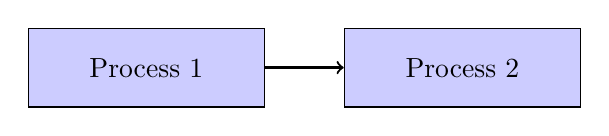
\begin{tikzpicture}[
    process/.style={rectangle, draw, fill=blue!20, minimum width=3cm, minimum height=1cm},
    arrow/.style={->, thick}
]

\node[process] (p1) {Process 1};
\node[process, right=of p1] (p2) {Process 2};

\draw[arrow] (p1) -- (p2);

\end{tikzpicture}
\end{document}